\section{Approach}
\label{sec:pi-approach}

% Barely from PUMPKIN Pi approach with a bit of intro

\toolnamec can do much more than permute constructors.
Given an equivalence between types \Aa and \B,
\toolnamec repairs functions and proofs defined over \Aa to instead refer to \B.
It does this in a way that allows for removing references to \Aa, which is essential for proof repair,
since \Aa may be an old version of an updated type.

The proof engineer can use \toolnamec (Section~\ref{sec:pi-workflow}) to automatically patch broken proofs in response to a broad class of changes in datatypes.
\toolnamec in particular repairs proofs in response to changes in types that correspond to \intro{type equivalences}~\cite{univalent2013homotopy},
or pairs of functions that map between two types (possibly with some additional information) and are mutual 
inverses (Section~\ref{sec:pi-scope}).\footnote{Every equivalence induces something called an \textit{adjoint} equivalence,
and those adjoint equivalences are nicer to work with.
\kl{Jasper} proved this fact for me in a way that does not rely on any axioms beyond those assumed by Coq~\href{https://github.com/uwplse/pumpkin-pi/blob/v2.0.0/plugin/theories/Adjoint.v}{\circled{23}},
and \kl{Nate} used that proof to build machinery for \toolnamec to derive the adjoint equivalence from the equivalence itself~\href{https://github.com/uwplse/pumpkin-pi/blob/v2.0.0/plugin/src/automation/search/equivalence.ml}{\circled{10}}.}
In other words, looking back to the thesis statement, the information shows up in the difference between versions of the changed datatype.
With automatic configuration, \toolnamec can extract and generalize that information to a type equivalence, then apply it to fix other broken proofs.
With manual configuration, the proof engineer extracts and generalizes the information corresponding to the change, but \toolnamec can still apply it
to fix other broken proofs.

Like the original \sysname prototype, \toolnamec also does this using a combination of differencing and proof term transformations.
The corresponding differencing algorithms (Section~\ref{sec:pi-spec-diff}) run in response to a breaking change in a datatype that corresponds to a type equivalence.
When they succeed, the diff that they find is that type equivalence.
The proof engineer can also pass the type equivalence to \toolnamec directly, effectively doing differencing by hand.
In either case, the proof term transformation (Section~\ref{sec:pi-spec-trans}) then transforms a proof term defined over the old version of the dataype
directly to a proof term defined over the new version of the datatype.
\toolnamec further supports proof script integration and other features for better workflow integration (Section~\ref{sec:pi-implementation}),
with real payoffs for proof engineers (Section~\ref{sec:pi-results}).

\subsection{Workflow: Configure, Transform, Decompile}
\label{sec:pi-workflow}

As with \sysname, the interface to \toolnamec is exposed to the proof engineer as a command.
\toolnamec extends \sysnamelong with a new command called \lstinline{Repair},
with the syntax:

\begin{lstlisting}
  Repair old_type new_type in old_proof.
\end{lstlisting}
where \lstinline{old_type} and \lstinline{new_type} are the old and new 
versions of the changed dataype, and \lstinline{old_proof} is the old version
of the proof broken by that change in datatype.
This invokes the \toolnamec plugin, which updates the old version of the proof to some new version of the proof
defined over the new version of the datatype, then defines it as a new proof term and suggests a corresponding new proof script if successful.
All terms that \toolnamec defines are type checked in the end, so \toolnamec does not extend the TCB.

\begin{figure}
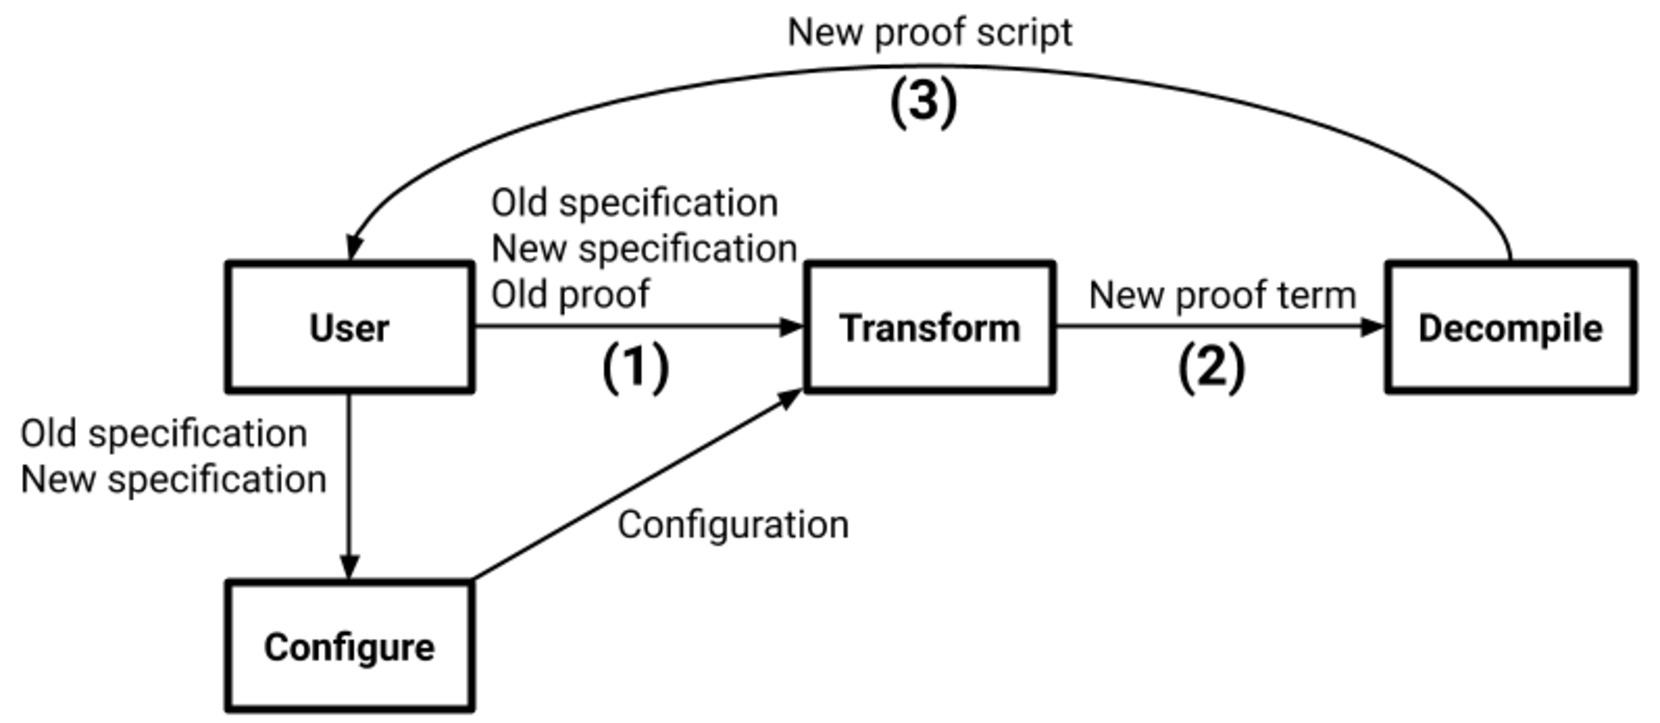
\includegraphics[width=\columnwidth]{often/workflowa.pdf}
\vspace{-0.7cm}
\caption{The workflow for \toolnamec.}
\vspace{-0.1cm}
\label{fig:system}
\end{figure}

Figure~\ref{fig:system} shows how this comes together when the proof engineer invokes \toolnamec:

\begin{enumerate}
\item The proof engineer \textbf{Configure}s \toolnamec, either manually or automatically.
\item The configured \textbf{Transform} transforms the old proof term into the new proof term.
\item \textbf{Decompile} suggests a new proof script. % given the new proof term.
\end{enumerate}
There are currently four search procedures for automatic configuration implemented in \toolnamec (see Table~\ref{fig:changes} on page~\pageref{fig:changes}).
Manual configuration makes it possible
for the proof engineer to configure the transformation to any equivalence,
even without a search procedure.

The breaking change to Figure~\ref{fig:listswap} in Section~\ref{pi:approach}, for example, used automatic configuration.
When we invoked \toolnamec:

\begin{lstlisting}
  Repair Old.list New.list in rev_app_distr.(@\vspace{-0.05cm}@)
\end{lstlisting}
it invoked a search procedure that differenced \lstinline{Old.list} and \lstinline{New.list},
then transformed \lstinline{rev_app_distr} to use \lstinline{New.list} in place of \lstinline{Old.list}.
In the end, it suggested a proof script to us that we could use going forward.

\subsection{Scope: Type Equivalences}
\label{sec:pi-scope}

\begin{figure*}
\codeauto{%
\begin{minipage}{0.48\textwidth}
\lstinputlisting[firstline=1, lastline=13]{often/equivproof.tex}
\end{minipage}
\hfill
\begin{minipage}{0.48\textwidth}
\lstinputlisting[firstline=15, lastline=28]{often/equivproof.tex}
\end{minipage}}
\vspace{-0.3cm}
\caption{Two functions between \lstinline{Old.list} and \lstinline{New.list} (top) that form an equivalence (bottom).}
\label{fig:equivalence}
\end{figure*}

\toolnamec automatically repairs proofs in response to changes in types that correspond to type equivalences.
When a type equivalence between types \Aa and \B exists, those types are \textit{equivalent} (denoted \Aa $\simeq$ \B). % for example:
Figure~\ref{fig:equivalence} shows a type equivalence between the two versions of \lstinline{list}
from Figure~\ref{fig:listswap} that \toolnamec discovered and proved automatically~\href{https://github.com/uwplse/pumpkin-pi/blob/v2.0.0/plugin/coq/Swap.v}{\circled{1}}.

To give some intuition for what kinds of changes can be described by equivalences, I preview two changes below.
See Table~\ref{fig:changes} on page~\pageref{fig:changes} for more examples.

\begin{figure}
\begin{minipage}{0.48\columnwidth}
\lstinputlisting[firstline=1, lastline=3]{often/equiv2.tex}
\end{minipage}
\hfill
\begin{minipage}{0.48\columnwidth}
\lstinputlisting[firstline=5, lastline=7]{often/equiv2.tex}
\end{minipage}
\vspace{-0.4cm}
\caption{The old type \lstinline{I} (left) is either \lstinline{A} or \lstinline{B}. The new type \lstinline{J} (right) is \lstinline{I} with \lstinline{A} and \lstinline{B} factored out to \lstinline{bool} (\codediff{orange}).}
\label{fig:equivalence2}
\end{figure}

\paragraph{Factoring out Constructors}
Consider changing the type \lstinline{I} to the type \lstinline{J} 
in Figure~\ref{fig:equivalence2}.
\lstinline{J} can be viewed as \lstinline{I} with its two constructors \lstinline{A} and \lstinline{B} pulled out to a
new argument of type \lstinline{bool} for a single constructor.
With \toolnamec, the proof engineer can repair functions and proofs about \lstinline{I} to instead use \lstinline{J},
as long as she configures \toolnamec to describe which constructor 
of \lstinline{I} maps to \lstinline{true} and which maps to \lstinline{false}.
This information about constructor mappings induces an equivalence \lstinline{I }$\simeq$\lstinline{ J}
across which \toolnamec repairs functions and proofs.
File \href{https://github.com/uwplse/pumpkin-pi/blob/v2.0.0/plugin/coq/playground/constr_refactor.v}{\circled{2}} shows an example of this, mapping \lstinline{A} to \lstinline{true} and \lstinline{B} to false,
and repairing proofs of De Morgan's laws. % constr_refactor.v
%
%It uses \toolnamec to automatically repair functions and proofs over \lstinline{I}, like:

%\begin{lstlisting}
%Theorem demorgan_1 : $\forall$ (i1 i2 : I),(@\vspace{-0.04cm}@)
%  neg (and i1 i2) = or (neg i1) (neg i2).(@\vspace{-0.04cm}@)
%Proof.(@\vspace{-0.04cm}@)
%  intros i1 i2.(@\vspace{-0.04cm}@)
%  induction i1; auto.(@\vspace{-0.04cm}@)
%Qed.
%\end{lstlisting}
%to corresponding functions and proofs over \lstinline{J}, like:
%
%\begin{lstlisting}[backgroundcolor=\color{cyan!30}]
%Theorem demorgan_1 : $\forall$ (j1 j2 : J),(@\vspace{-0.04cm}@)
%  neg (and j1 j2) = or (neg j1) (neg j2).(@\vspace{-0.04cm}@)
%Proof.(@\vspace{-0.04cm}@)
%  intros j1 j2.(@\vspace{-0.04cm}@)
%  induction j1 (@\codediff{as [b]. induction b as [ | ]}@); auto.(@\vspace{-0.04cm}@)
%Qed.
%\end{lstlisting}
%These repaired functions and proofs refer to \lstinline{J} in place of \lstinline{I}.
%Otherwise, they behave the same way as the functions and proofs over \lstinline{I} up to the equivalence between
%\lstinline{I} and \lstinline{J}---Section~\ref{sec:repair} explains this intuition more formally.

\begin{figure}
\begin{minipage}{0.48\textwidth}
   \lstinputlisting[firstline=1, lastline=3]{often/listtovect.tex}
\end{minipage}
\hfill
\begin{minipage}{0.58\textwidth}
   \lstinputlisting[firstline=5, lastline=7]{often/listtovect.tex}
\end{minipage}
\vspace{-0.4cm}
\caption{A vector (bottom) is a list (top) indexed by its length (\codediff{orange}). Vectors effectively make it possible to enforce length invariants about lists at compile time.}
\label{fig:listtovect}
\end{figure}

\paragraph{Adding a Dependent Index}
At first glance, the word \textit{equivalence} may seem to imply that \toolnamec can support only changes in
which the proof engineer does not add or remove information.
But equivalences are more powerful than they may seem.
%The idea is, when possible, to separate out the new information
%into a projection of a $\Sigma$ type or a constructor of a sum type.
%roofs about this new information become the proof obligation for the proof engineer,
%and \toolnamec automates the rest.
Consider, for example, changing a list to a length-indexed vector (Figure~\ref{fig:listtovect}).
\toolnamec can repair functions and proofs about lists to functions and proofs about vectors of particular lengths~\href{https://github.com/uwplse/pumpkin-pi/blob/v2.0.0/plugin/coq/examples/Example.v}{\circled{3}}, % Example.v
since $\Sigma$\lstinline{(l:list T).length l = n }$\simeq$\lstinline{ vector T n}.
From the proof engineer's perspective, after updating specifications from \lstinline{list} to \lstinline{vector},
to fix her functions and proofs, she must additionally prove invariants about the lengths of her lists.
\toolnamec makes it easy to separate out that proof obligation, then automates the rest.

More generally, in homotopy type theory, with the help of quotient types, it is possible to form an equivalence
from a relation, even when the relation is not an equivalence~\cite{angiuli2020internalizing}.
While Coq lacks quotient types,
it is possible to achieve a similar outcome and use \toolnamec for changes that add or remove information
when those changes can be expressed as equivalences between $\Sigma$ types or sum types.

\subsection{Differencing: Equivalences from Changes}
\label{sec:pi-spec-diff}

Differencing in \toolnamec is what configures the proof term transformation with a particular type equivalence.
By default, when the proof engineer invokes the \lstinline{Repair} command, differencing runs automatically.
For example, when we invoked:

\begin{lstlisting}
  Repair Old.list New.list in rev_app_distr.(@\vspace{-0.05cm}@)
\end{lstlisting}
in Section~\ref{pi:approach}, differencing discovered and proved the equivalence in Figure~\ref{fig:equivalence}.
In total, \toolnamec currently implements four search procedures for automatic configuration;
I will explain these more in Sections~\ref{sec:pi-diff} and~\ref{sec:pi-implementation}.
Each search procedure automates differencing for an entire class of changes that correspond to type equivalences. 
In the end, it returns a configuration that corresponds to the equivalence (see Section~\ref{sec:pi-diff} for details),
along with the equivalence itself.

Manual configuration makes it possible for the proof engineer to skip differencing, so that \toolnamec is not limited by the 
search procedures currently implemented.
Manual configuration supports any change that can be described by a type equivalence.
To configure \toolnamec manually, the proof engineer can pass the configuration correspond to the equivalence to \toolnamec's \lstinline{Configure Repair} command before invoking \lstinline{Repair}.
This is what I did for the change in Figure~\ref{fig:equivalence2} \href{https://github.com/uwplse/pumpkin-pi/blob/v2.0.0/plugin/coq/playground/constr_refactor.v}{\circled{2}}.

\paragraph{Summary}

In summary, differencing has the following specification:

\begin{itemize}
\item \textbf{Inputs}: types \Aa\ and \B, assuming:
\begin{itemize}
\item there is a type equivalence describing the change from \Aa to \B (possibly with some new information), and
\item the corresponding change is in a class currently supported by a search procedure for automatic configuration.
\end{itemize}
\item \textbf{Outputs}:
\begin{itemize}
\item functions \lstinline{f} and \lstinline{g},
\item proofs \lstinline{section} and \lstinline{retraction}, and
\item a configuration $c$,
\end{itemize}
guaranteeing:
\begin{itemize}
\item \lstinline{f} and \lstinline{g} form an equivalence that describes the change from \Aa to \B (possibly with some new information),
\item \lstinline{section} and \lstinline{retraction} prove that \lstinline{f} and \lstinline{g} form an equivalence, and
\item $c$ is a decomposition of the equivalence.
\end{itemize}
\end{itemize}
The new information for the change in Figure~\ref{fig:listtovect}, for example, is the length of the list.
Differencing discovers the equivalence corresponding to this change, as well as a configuration $c$ that is a decomposition of this equivalence.
Section~\ref{sec:pi-diff} describes what it means for $c$ to be a decomposition of the equivalence,
and proves that this is possible for any equivalence.
Manual configuration, on the other hand, takes in the configuration directly.
In either case, the transformation uses this configuration to automatically repair broken proofs.

 % TODO in impl, note that it's not quite just automatic and manual, but actually some automatic configurations take human guidance

\subsection{Transformation: Transport with a Twist}
\label{sec:pi-spec-trans}

\toolnamec repairs proofs in response to these changes by implementing a kind of proof reuse known as \textit{transport}~\cite{univalent2013homotopy},
but in a way that is suitable for repair.
Informally, transport takes a term $t$ and produces a term $t'$ that is the same as $t$ modulo an equivalence $A \simeq B$.
If $t$ is a function, then $t'$ behaves the same way modulo the equivalence;
if $t$ is a proof, then $t'$ proves the same theorem the same way modulo the equivalence.

When transport across $A \simeq B$ takes $t$ to $t'$,
I say that $t$ and $t'$ are \textit{equal up to transport}
across that equivalence (denoted $t \equiv_{A \simeq B} t'$).\footnote{This notation should be interpreted in a metatheory with \textit{univalence}---a property that Coq lacks---or it should be approximated in Coq.
The details of transport with univalence are in the Homotopy Type Theory book~\cite{univalent2013homotopy}, and an approximation in Coq is in the univalent parametricity framework paper~\cite{tabareau2017equivalences}. For equivalent \Aa and \B, there can be many equivalences $A \simeq B$.
Equality up to transport is across a \textit{particular} equivalence, but I erase this in the 
notation.}
In Section~\ref{sec:overview}, the original append function \lstinline{++} over \lstinline{Old.list}
and the repaired append function \lstinline{++} over \lstinline{New.list} that \toolnamec produces are
equal up to transport across the equivalence from Figure~\ref{fig:equivalence}, since (by \lstinline{app_ok}~\href{https://github.com/uwplse/pumpkin-pi/blob/v2.0.0/plugin/coq/Swap.v}{\circled{1}}):

\begin{lstlisting}
  $\forall$ T (l1 l2 : Old.list T),(@\vspace{-0.04cm}@)
    swap T (l1 ++ l2) = (swap T l1) ++ (swap T l2).(@\vspace{-0.05cm}@)
\end{lstlisting}
The original \lstinline{rev_app_distr} is equal to the repaired proof up to transport,
since both prove the same thing the same way up to the equivalence, and up to the changes in \lstinline{++}
and \lstinline{rev}.

Transport typically works by applying the functions that make up the equivalence to convert
inputs and outputs between types.
This approach would not be suitable for repair, since it does not make it possible to remove the old type \Aa.
\toolnamec implements transport in a way that allows for removing references to \Aa---by proof term transformation.

\paragraph{Summary}

In summary, the transformation has the following specification:

\begin{itemize}
\item \textbf{Inputs}:
\begin{itemize}
\item types \Aa\ and \B,
\item the configuration $c$, and
\item a proof term $t$,
\end{itemize}
assuming $c$ corresponds to a type equivalence describing the change from \Aa to \B (possibly with some new information).
\item \textbf{Outputs}: a proof term $t'$, guaranteeing:
\begin{itemize}
\item \smallmath{$t'$} refers to \B in place of \Aa, and
\item $t$ and $t'$ are equal up to transport along the equivalence formed by $c$.
\end{itemize}
\end{itemize}
This specification glazes over a few important issues, most notably that \B may refer to \Aa (so \toolnamec has specialized termination logic),
and that it may be desirable to port only \textit{some} instances of \Aa to \B (but \toolnamec by default ports \textit{all} instances). 
I discuss these more in Sections~\ref{sec:pi-trans} and~\ref{sec:pi-implementation}.

